\subsection{Loss Graphs}

\subsubsection{Learning Rate}

    \begin{figure}[H]
        \minipage{0.5\textwidth}
        \includegraphics[width=\linewidth]{testsResults/loss/lr/def.png}
        \caption{Default settings + learning rate = 0.001}
        \endminipage\hfill
        \minipage{0.5\textwidth}
        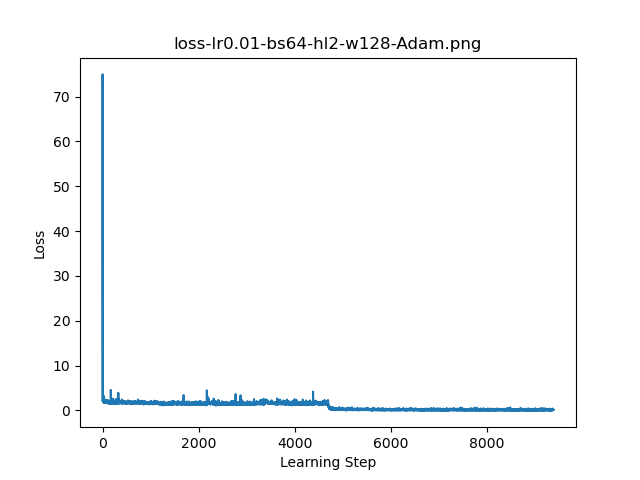
\includegraphics[width=\linewidth]{testsResults/loss/lr/loss-lr0.01-bs64-hl2-w128-Adam.png}
        \caption{Default settings + learning rate = 0.01}
        \endminipage
    \end{figure}
        \begin{figure}[H]
        \minipage{0.5\textwidth}%
        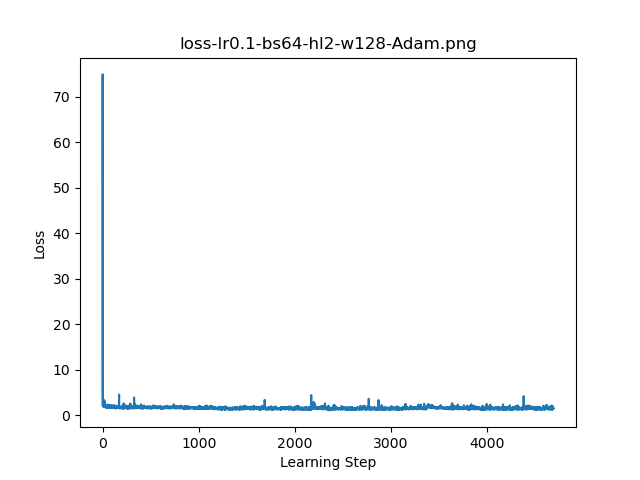
\includegraphics[width=\linewidth]{testsResults/loss/lr/loss-lr0.1-bs64-hl2-w128-Adam.png}
        \caption{Default settings + learning rate = 0.1}
        \endminipage
    \end{figure}

    \paragraph{Analysis} Smaller learning rate causes losses to drop near zero level faster (notice how there is a vertical drop for lower learning step for leaerning rate 0.001, later for learning rate 0.01 and never for learnig rate 0.1) 

\subsubsection{Mini-Batch size}

    \begin{figure}[H]
        \minipage{0.5\textwidth}
        \includegraphics[width=\linewidth]{testsResults/loss/bs/def.png}
        \caption{Default settings + batching size = 64}
        \endminipage\hfill
        \minipage{0.5\textwidth}
        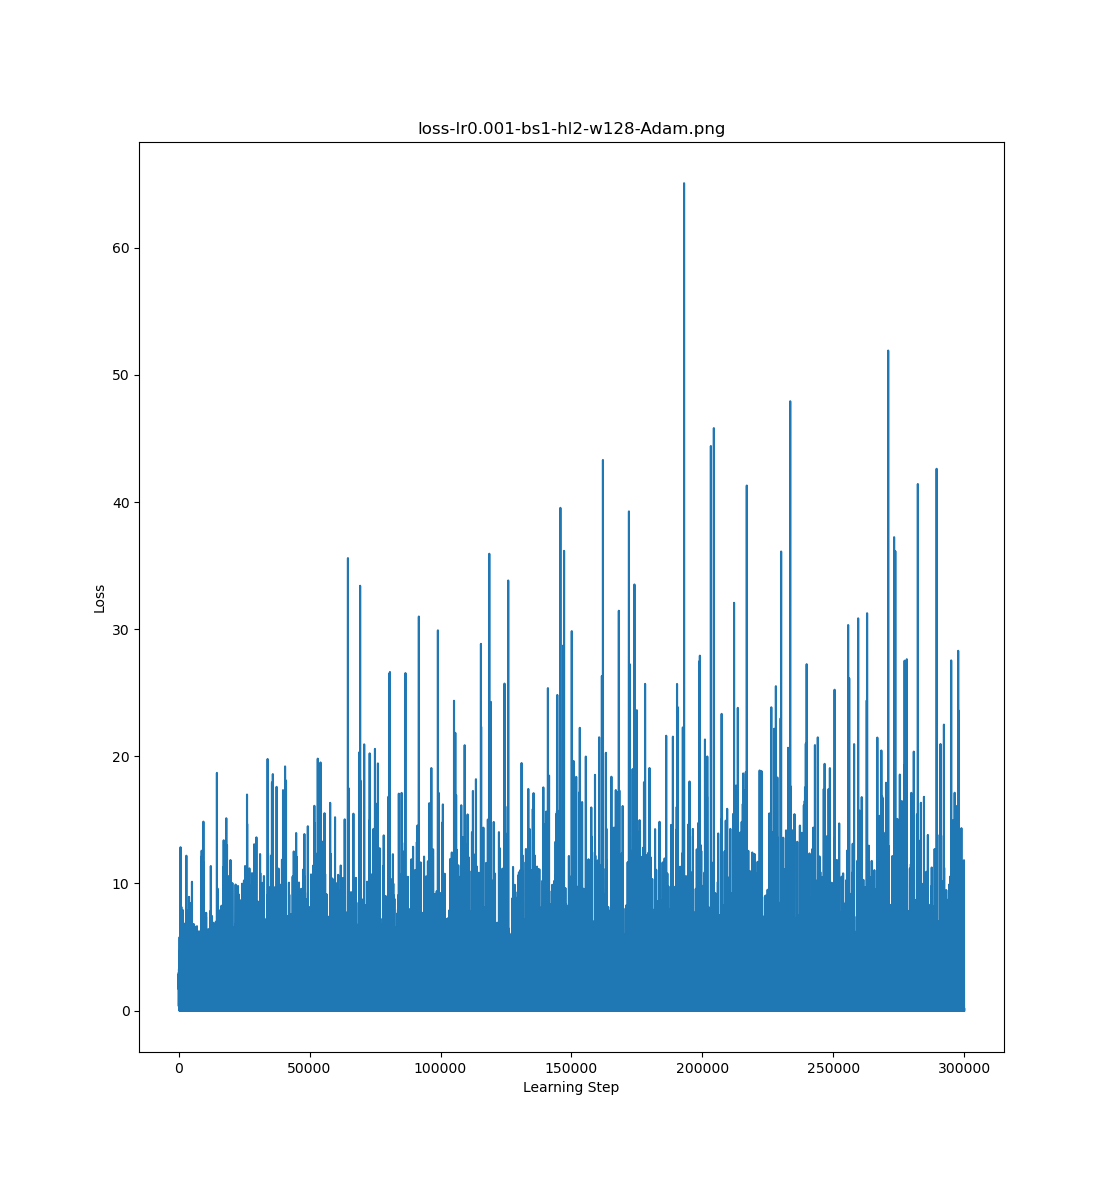
\includegraphics[width=\linewidth]{testsResults/loss/bs/loss-1batch.png}
        \caption{Default settings + batching size = 1}
        \endminipage
    \end{figure}
        \begin{figure}[H]
        \minipage{0.5\textwidth}%
        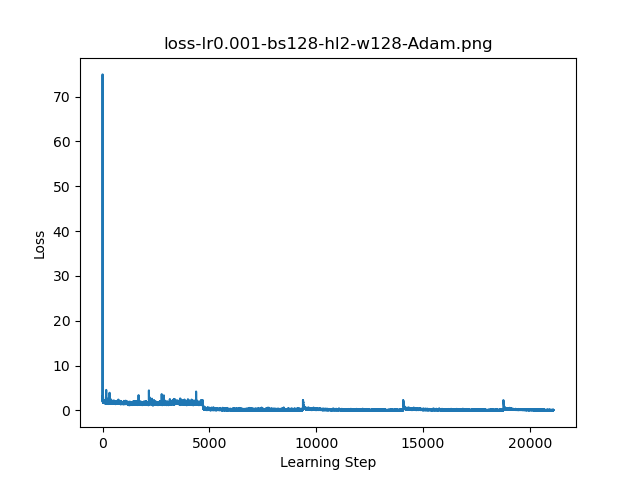
\includegraphics[width=\linewidth]{testsResults/loss/bs/loss-lr0.001-bs128-hl2-w128-Adam.png}
        \caption{Default settings + batching size = 128}
        \endminipage
        \minipage{0.5\textwidth}%
        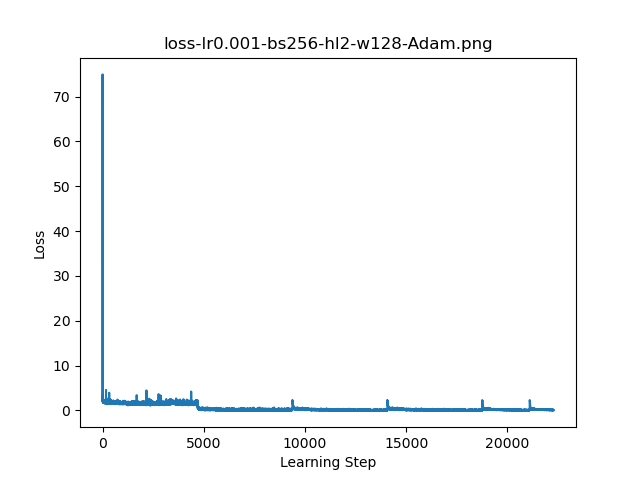
\includegraphics[width=\linewidth]{testsResults/loss/bs/loss-lr0.001-bs256-hl2-w128-Adam.png}
        \caption{Default settings + batching size = 256}
        \endminipage
    \end{figure}

    \paragraph{Analysis} Batching size equal to 1 makes losses seem pretty much random, increasing batch sizes increases 'flat' (smaller) loss periods between local peaks

\subsubsection{Number of Hidden Layers}

    \begin{figure}[H]
        \minipage{0.5\textwidth}
        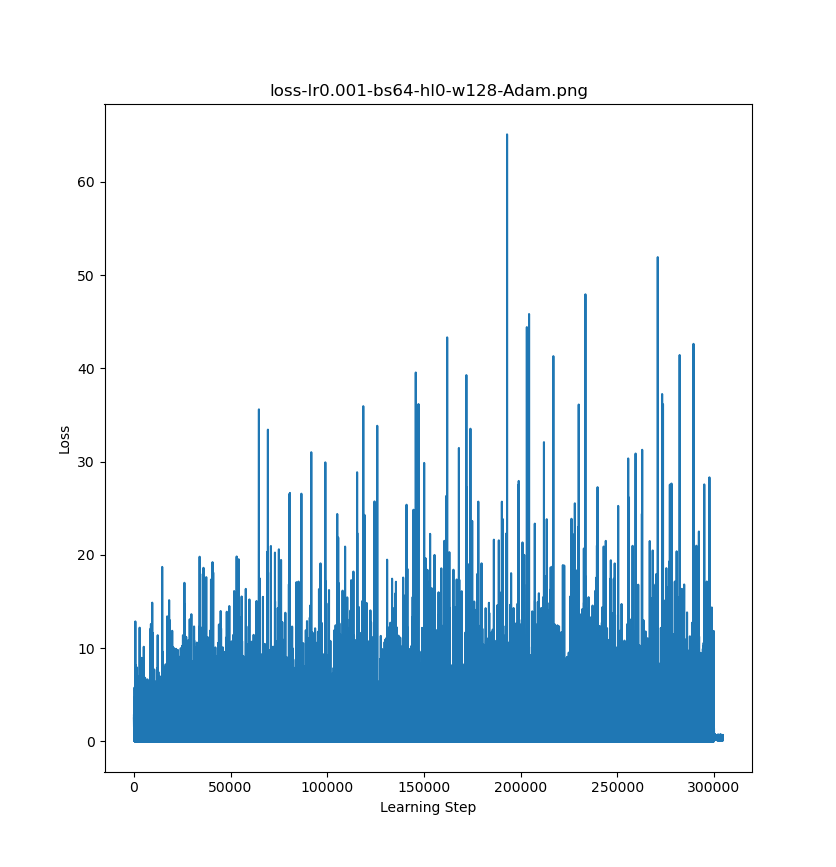
\includegraphics[width=\linewidth]{testsResults/loss/hl/hl0loss.png}
        \caption{Default settings + hidden layers = 0}
        \endminipage\hfill
        \minipage{0.5\textwidth}
        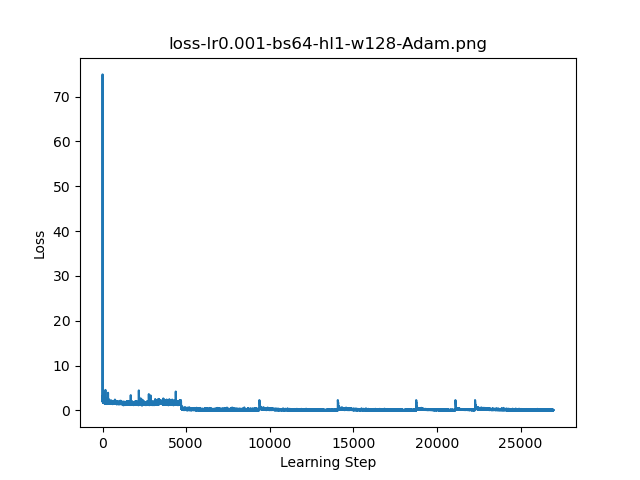
\includegraphics[width=\linewidth]{testsResults/loss/hl/loss-lr0.001-bs64-hl1-w128-Adam.png}
        \caption{Default settings + hidden layers = 1}
        \endminipage
    \end{figure}
        \begin{figure}[H]
        \minipage{0.5\textwidth}%
        \includegraphics[width=\linewidth]{testsResults/loss/hl/def.png}
        \caption{Default settings + hidden layers = 2}
        \endminipage
        \minipage{0.5\textwidth}%
        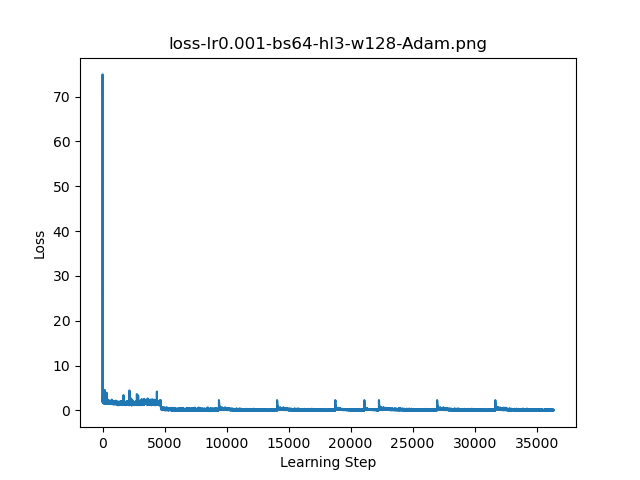
\includegraphics[width=\linewidth]{testsResults/loss/hl/loss-lr0.001-bs64-hl3-w128-Adam.png}
        \caption{Default settings + hidden layers = 3}
        \endminipage
    \end{figure}

    \paragraph{Analysis} Setting hidden layers to 0 again makes losses value seem random, hidden layer set to 1 provides us with later drop but longer flat periods, number of hidden layers set to 2 offeres the opposite and number of layers set to 3 seems to be a compromise between those two 
\subsubsection{Width}

    \begin{figure}[H]
        \minipage{0.5\textwidth}
        \includegraphics[width=\linewidth]{testsResults/loss/w/def.png}
        \caption{Default settings + width = 128}
        \endminipage\hfill
        \minipage{0.5\textwidth}
        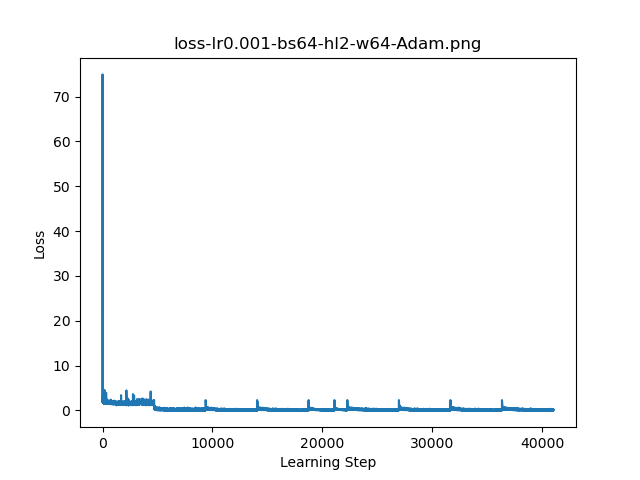
\includegraphics[width=\linewidth]{testsResults/loss/w/loss-lr0.001-bs64-hl2-w64-Adam.png}
        \caption{Default settings + width = 64}
        \endminipage
    \end{figure}
        \begin{figure}[H]
        \minipage{0.5\textwidth}%
        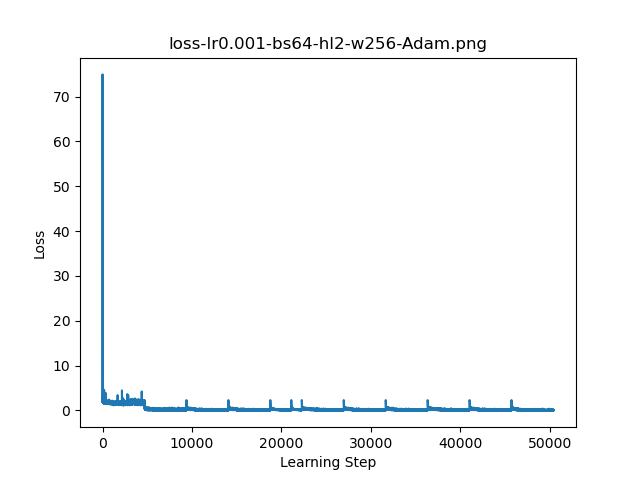
\includegraphics[width=\linewidth]{testsResults/loss/w/loss-lr0.001-bs64-hl2-w256-Adam.png}
        \caption{Default settings + width = 256}
        \endminipage
        \minipage{0.5\textwidth}%
        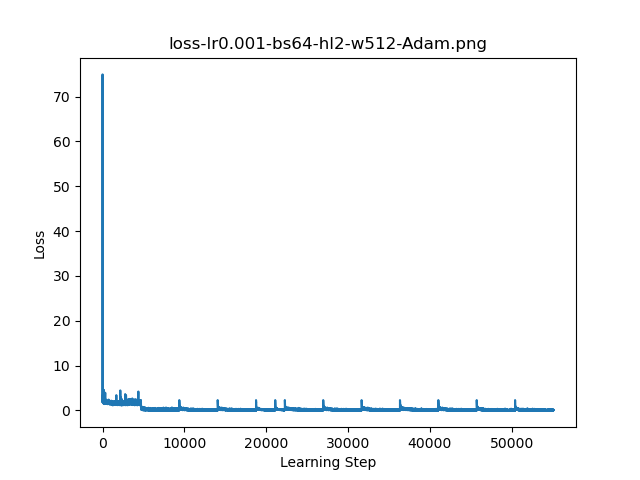
\includegraphics[width=\linewidth]{testsResults/loss/w/loss-lr0.001-bs64-hl2-w512-Adam.png}
        \caption{Default settings + width = 512}
        \endminipage
    \end{figure}
    \begin{figure}[H]
        \minipage{0.5\textwidth}%
        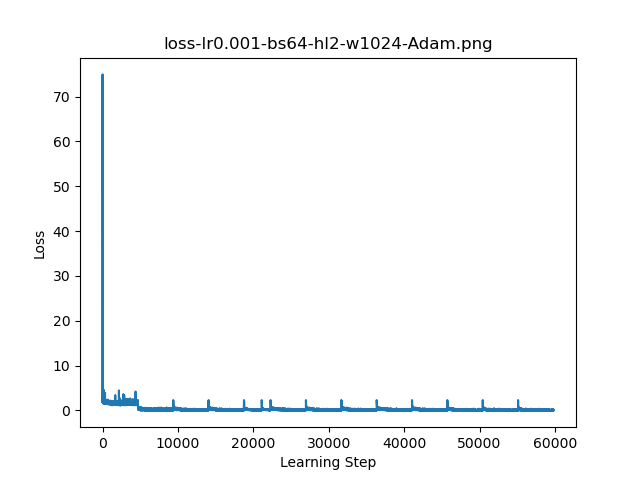
\includegraphics[width=\linewidth]{testsResults/loss/w/loss-lr0.001-bs64-hl2-w1024-Adam.png}
        \caption{Default settings + width = 1024}
        \endminipage
    \end{figure}

    \paragraph{Analysis} Changing width does not seem to affect loss greatly


\subsubsection{Optimizer Type}

    \begin{figure}[H]
        \minipage{0.5\textwidth}
        \includegraphics[width=\linewidth]{testsResults/loss/optimizer/def.png}
        \caption{Default settings + Adam optimizer}
        \endminipage\hfill
        \minipage{0.5\textwidth}
        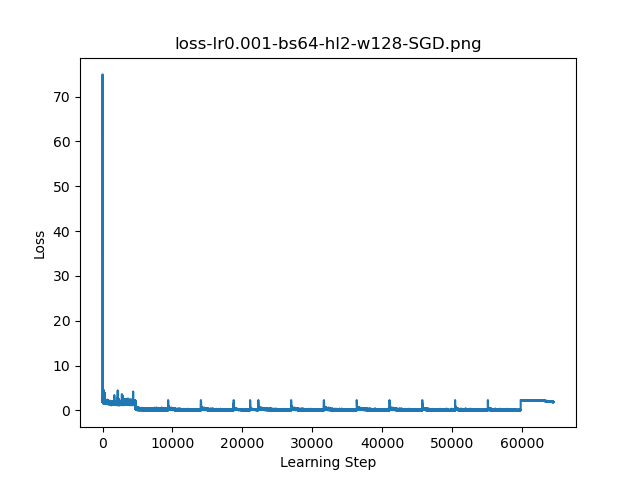
\includegraphics[width=\linewidth]{testsResults/loss/optimizer/loss-lr0.001-bs64-hl2-w128-SGD.png}
        \caption{Default settings + learning rate = 0.01}
        \endminipage
    \end{figure}
        \begin{figure}[H]
        \minipage{0.5\textwidth}%
        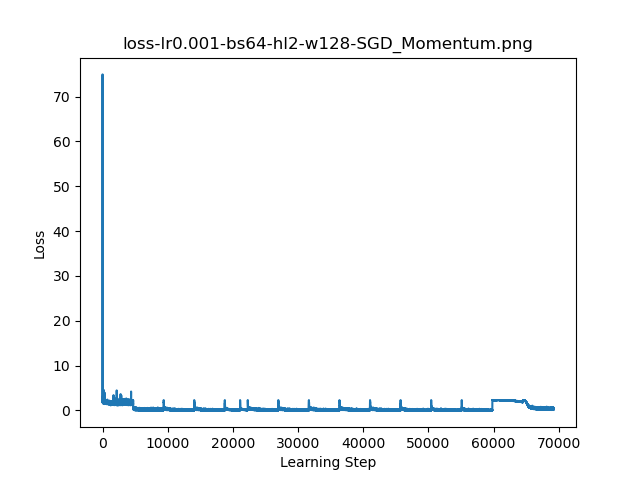
\includegraphics[width=\linewidth]{testsResults/loss/optimizer/loss-lr0.001-bs64-hl2-w128-SGD_Momentum.png}
        \caption{Default settings + SGD\_Momentum optimizer}
        \endminipage
    \end{figure}

    \paragraph{Analysis} Changing optimizers does not seem to affect loss greatly


